\jxhj{%教学后记
	}
\skrq{%授课日期
	2017年10月19日 4-5节}
\ktmq{%课题名称
	 子程序的XY向分层}
\jxmb{%教学目标,每行前面要加 \item
	\item 掌握子程序指令的使用;
	\item 掌握用子程序编程;
	\item 掌握用子程序及刀补实现XY向分层;
	\item 掌握子程序的嵌套调用。 }	
\jxzd{%教学重点,每行前面要加 \item
	\item 用子程序及刀补实现XY向分层;
	\item 子程序的嵌套调用。 }
\jxnd{%教学难点,每行前面要加 \item
	\item 用子程序及刀补实现XY向分层。 }
\jjff{%教学方法
	通过讲述、举例、演示法来说明;}

\makeshouye %制作教案首页

%%%%教学内容
\subsection{组织教学}
\begin{enumerate}[\hspace{2em}1、]
	\item 集中学生注意力;
	\item 清查学生人数;
	\item 维持课堂纪律;
\end{enumerate}
\subsection{复习导入及主要内容}
\begin{enumerate}[1、]
	\item 子程序的概念;
\item 子程序的组成;
\item 子程序的调用;
\item 子程序的使用。
\end{enumerate}


\subsection{教学内容及过程}

\subsubsection{加工实例分析}

如图\ref{fig:11-1}所示:加工凸台零件,高12mm。

\begin{figure}[h]
	\centering
	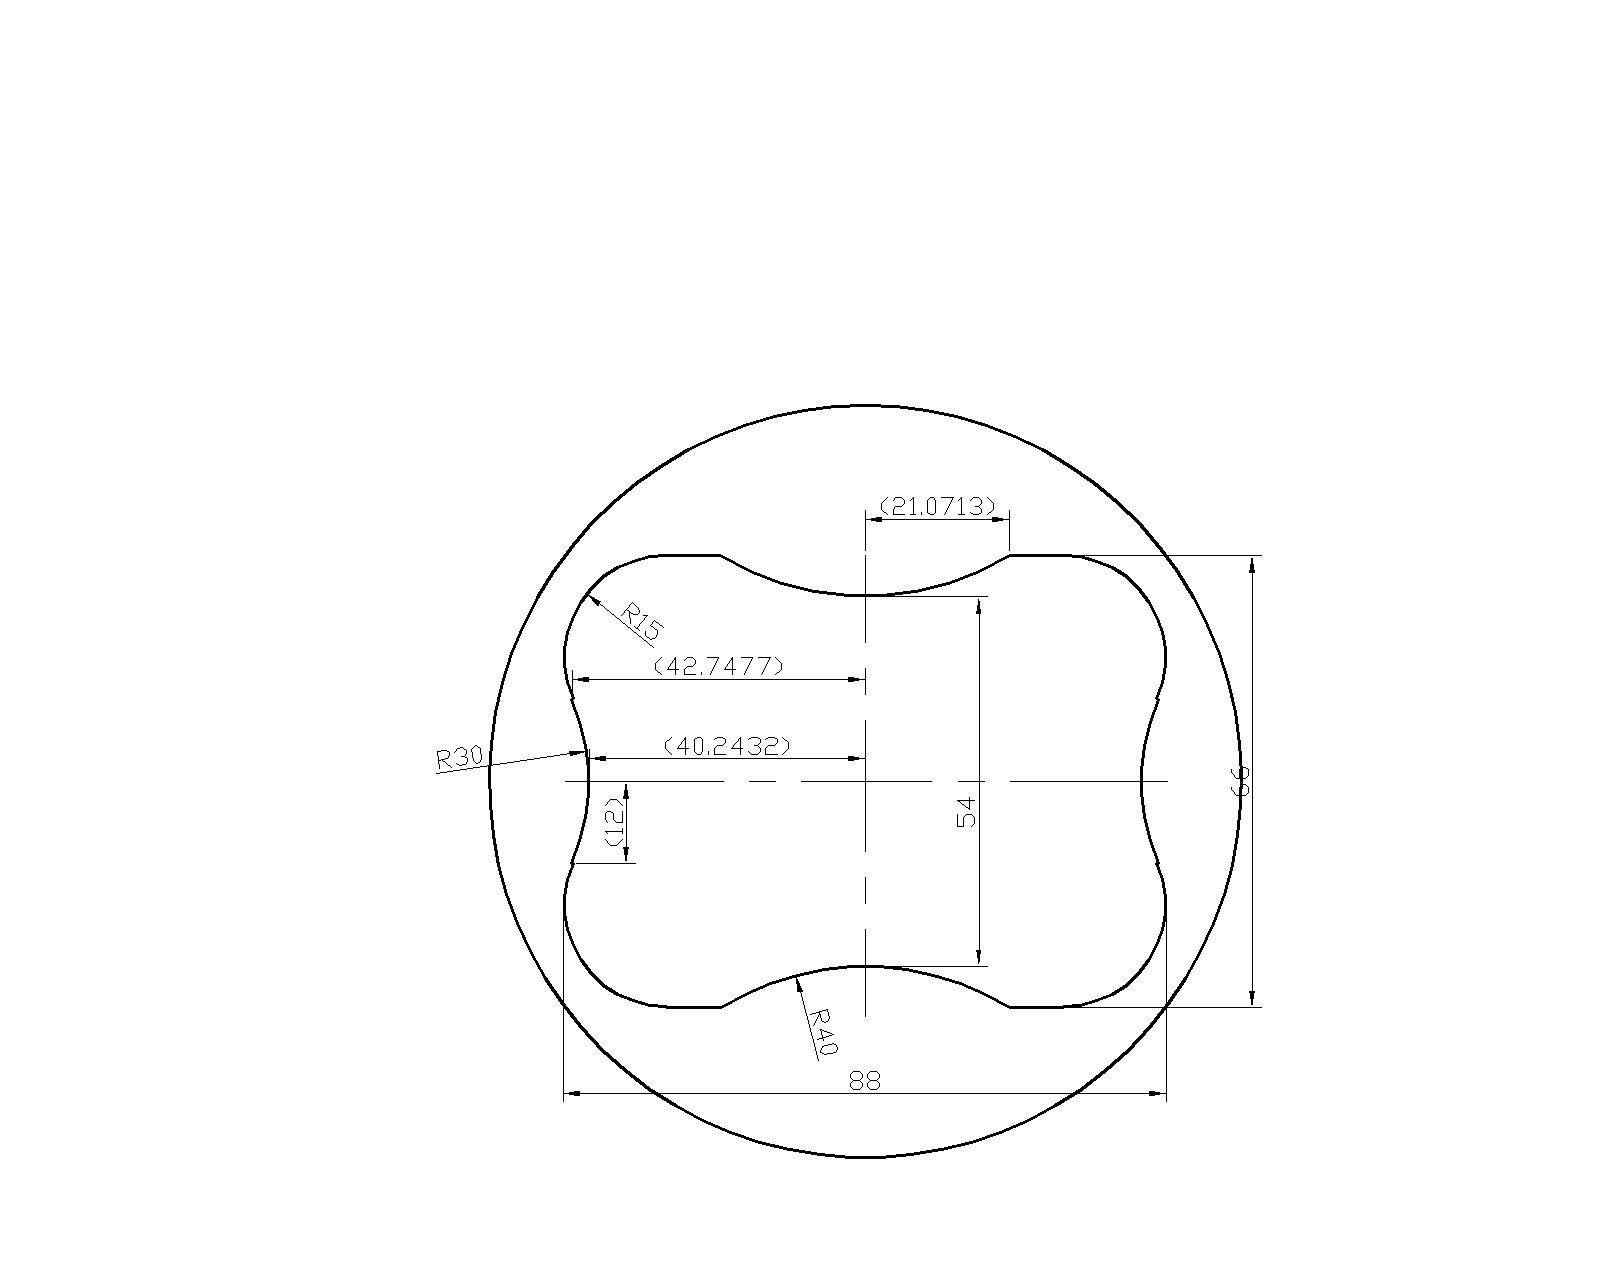
\includegraphics[width=0.7\linewidth,trim=250 50 150  250,clip]{data/image/11-1.jpg}
	\caption{刀补实例}
	\label{fig:11-1}
\end{figure}

毛坯:\diameter 110*35

刀具:\diameter 12立铣刀

1、Z向分层加工:

高12mm     3mm*4次     深度等分下刀

用G91 G01 Z-3.0 F300; Z方向要先定好位

是Z方向

2、XY向分层,平面上的等分铣削:

方法:用不同的刀具半径值:

A、刀具补偿值的确定:(由小到大确定)

大=较大+B

较大=小+B

小=D/2+(0.2-0.6)

B=50-80\% *D 

判断是否把多余材料去完

B、切入/切出圆弧半径:

R>最大的刀补值

C、XY平面内的定位

第一次铣削后,刀具位置应回到原来位置

3、参考程序:

主程序:


\begin{lstlisting}
O0001
G54 G17 G40 G49 G90
M03 S300
G01 X0 Y75.0 F800
Z0
M98 P40002
G01 Z30.0
M05
M30
\end{lstlisting}

下刀子程序
\begin{lstlisting}
O0002
G91 G01 Z-3.0 
G90
D1 M98 P3
D2 M98 P3
D3 M98 P4
M99
\end{lstlisting}
轮廓子程序
\begin{lstlisting}
O0003
G41 G01 X-40.0 Y67.0
G03 X21.071 Y33.0 R40.0
G1 X39
G03 X42.748 Y12.0 R15.0
G02 Y-12.0 R30.0
G03 X39 Y-33.0 R15.0
G01 X21.071
G03 X-21.071 R40.0
G01 X-39.0
G03 X-42.748 Y-12.0 R15.0
G02 Y12.0 R30.0
G03 X-39.0 Y33.0 R15.0
G01 X-21.071 
G03 X40.0 Y67.0 R40.0
G40 G01 X0 Y75.0
M99
\end{lstlisting}

\subsubsection{使用子程序的场合}
1、同一零件上有重复加工的部位

2、批量加工,一次加工多个相同的工件

3、同一个零件上有多个不同形状的加工轮廓

可使程序看起来方便,简单

不使用的场合:

自动编程不用子程序:

1、多程序传输不方便

2、自动编程子程序完成后,修改的内容多。

\subsection{课堂小结}
\begin{enumerate}[1、]
	\item 子程序Z向分层;
	\item 子程序XY向分层;
	\item 子程序的应用。	
\end{enumerate}

\vfill
\subsection{布置作业}
\begin{enumerate}[1、]
	\item 用子程序编写一个Z向分层+XY向分层的程序。 
\end{enumerate}
\vfill